\chapter{Overall description}

\section{Product perspective}

\subsection{Scenarios}

In the following chapter, we present a hypothetical scenario to better illustrate the phenomenon:

\begin{itemize}[leftmargin=*, label={}]
    \item \textbf{Quahog Innovation Company inserts an internship:}
    \begin{itemize}
        \item The Quahog Innovation Company, a leader in Integrating AI into different infrastructures, seeks interns who can bring fresh perspectives to their research. Upon learning about the S\&C platform, they decide to list their internship opportunity there, hoping to attract enthusiastic candidates eager to collaborate. 
    \end{itemize}

    \item \textbf{Quahog Innovation Company improves its internship proposal:}
    \begin{itemize}
        \item As this is the first time the Quahog  Innovation Company is offering an internship, they are unsure how appealing their proposal might be. They follow the platform's suggestions to post first and then enhance their posting, aiming to make it more attractive to potential applicants.
    \end{itemize}

    \item \textbf{Stewie registers on the platform:}
    \begin{itemize}
        \item Stewie, a master’s student at Cleveland University, needs an internship related to his field of study to support his thesis. After discovering the S\&C platform, he decides to use it to find opportunities. He follows the app’s guidance to make his CV and personal account. In the end, he is not convinced about the attractiveness of his curriculum and decides to improve it by following the platform’s guidance to make it more compelling.
    \end{itemize}

    \item \textbf{Stewie applies for an internship:}
    \begin{itemize}
        \item  Once satisfied with the improvements, he starts applying to several internships that not only match his academic background but also fit his interests and long-term career goals, hoping to gain valuable experience that will support his thesis and future aspirations.
    \end{itemize}

    \item \textbf{Quahog Innovation Company analyses the applications received:}
    \begin{itemize}
        \item After receiving multiple applications, the Quahog  Innovation Company begins evaluating candidates. They first filter out applicants who do not meet the prerequisites. Next, they assess the level of interest shown by the remaining candidates, ultimately shortlisting those they believe would bring the greatest value to their organization and match them.
    \end{itemize}

    \item \textbf{Stewie Checks the Status of His Applications:}
    \begin{itemize}
        \item Stewie monitors his applications and finds that while some companies have shown no interest, others have matched him. He also received notifications about new internship opportunities. However, he chooses to proceed with the companies that have expressed interest in his application, as they align better with his aspirations.
    \end{itemize}

    \item \textbf{The company evaluates and interviews applicants:}
    \begin{itemize}
        \item To finalize their decision, the company interviews the students through a structured questionnaire for each specific internship proposed, which all shortlisted candidates have to answer if accepted. In order to make a more The interview delves into the technical knowledge required for the role and asks personal questions about their motivations and goals. Candidates respond to the questionnaire through the platform, providing the company with deeper insights.
    \end{itemize}

    \item \textbf{Stewie receives the questionnaire and answers it}
    \begin{itemize}
        \item Stewie while checking the status of his application notices that the one to Quohag Company was positively evaluated and a questionnaire was available to be answered. Excited about the news, Stewie immediately answers all the questions present and sends back the questionnaire, hoping that the company will continue to show interest in him. 
    \end{itemize}

    \item \textbf{The company evaluates the questionnaires and hires the interns:}
    \begin{itemize}
        \item After reviewing the questionnaires submitted, Quahog Innovation Company identifies candidates who demonstrate technical skills and a passion for AI integration. Following a thorough evaluation, the company shortlists the candidates they want to hire, including Stewie.
    \end{itemize}

    \item \textbf{Stewie accepts the position and starts working in the company:}
    \begin{itemize}
        \item Stewie receives a notification stating that his questionnaire was evaluated positively and that if interested would be contacted by the company with the messaging system available on the platform. Extremely excited, he accepts and gets contacted by the company to clarify all the final information needed before finally starting his experience at Quohag company.
    \end{itemize}

    \item \textbf{Complaints handling:}
    \begin{itemize}
        \item After starting to work at the company, Stewie noticed a few issues with his internship. As time passes, instead of engaging in meaningful work that aligned with his skills and interests, he was assigned only trivial tasks that seemed far beneath his aspirations. Frustrated by the lack of stimulation, Stewie raises a complaint on the S\&C platform. The Cleveland University administration steps in to mediate, contacting the company to address the issue. Prompted by the intervention, the company apologizes and puts Stewie on a new project much closer to his field of interest.
    \end{itemize}
        
    \item \textbf{Finalizing the decision:}
    \begin{itemize}
        \item With the issues resolved, Stewie feels reassured and continues the internship. Excited to start this new project, he leaves a good review on the platform and looks forward to contributing to the company’s innovative projects while gathering valuable information for his thesis and academic growth.
    \end{itemize}
\end{itemize}


\subsection{Domain Class Diagram}

\begin{figure} [H]
    \centering
    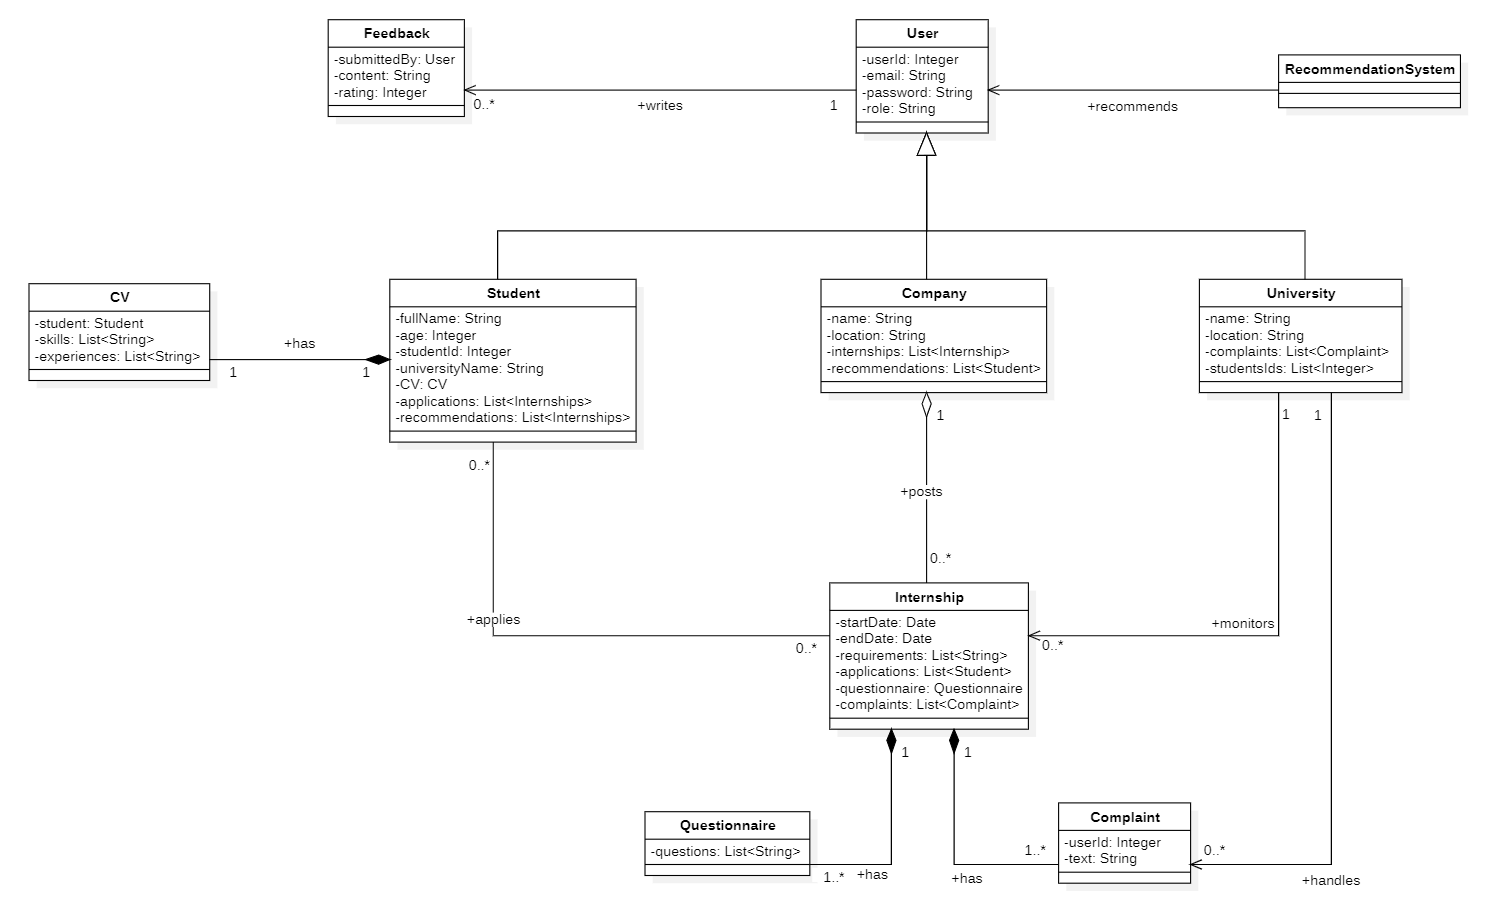
\includegraphics[width=1\linewidth]{Images/domain_class_diagram.png}
    \caption{High level Class Diagram}
    \label{fig: High level Class Diagram}
\end{figure}

\section{Product Functions}

The S\&C platform provides a range of functionalities designed to support the internship matching process for students and companies, oversighted by universities. The main functionalities are described below.

\subsubsection*{User Registration} 
This functionality allows students, companies, and universities to sign up to the S\&C platform and create their profiles.
\begin{itemize}
    \item \textbf{User}: Each user selects their type (student, company, or university) and provides the required information to complete the registration process, such as email, password, and other relevant details.
\end{itemize}

\subsubsection*{Profile Management} 
This functionality enables users to manage and enhance their profiles to increase the likelihood of successful matches.
\begin{itemize}
    \item \textbf{Profile Updates}: Students and companies can update their personal information to complete their profiles after registration.
    \item \textbf{CV Creation}: Students can generate their CVs by providing details about their skills, personal experiences, and other relevant information.
\end{itemize}

\subsubsection*{Enhancement Suggestions}
This feature helps both students and companies improve their profiles and increase their chances to make themselves more appealing to potential matches.
\begin{itemize}
    \item \textbf{CV Improvement}: Students can request suggestions from the system to improve their CVs.
    \item \textbf{Internship Improvement}: Companies can request suggestions from the system to enhance their internship proposals.
    \item \textbf{Questionnaire Improvement}: Companies can request suggestions to improve their questionnaires.
\end{itemize}

\subsubsection*{Internship Posting and Search} 
The platform allows companies to post internships and students to search for opportunities.
\begin{itemize}
    \item \textbf{Internship Creation}: Companies can create detailed internship listings by specifying requirements, skills needed, tasks, compensation, and benefits.
    \item \textbf{Internship Search and Filtering}: Students can browse and filter internships based on criteria such as required skills, duration, location, and compensation.
    \item \textbf{Internship Details View}: Students can thoroughly view details about each internship to assess compatibility with their skills and interests.
\end{itemize}

\subsubsection*{Application and Selection Process} 
This functionality manages applications and the selection process.
\begin{itemize}
    \item \textbf{Application Submission}: Students can apply to internships directly from the listings and track the status of their applications.
    \item \textbf{Candidate Shortlisting}: Companies can review applications, filter candidates based on qualifications, and shortlist those who meet their requirements.
    \item \textbf{Interview Coordination}: Companies can arrange interviews with shortlisted candidates by using questionnaires.
    \item \textbf{Final Selection and Offer Acceptance}: Companies can send offers to selected students, who can accept or decline the offers through the platform.
\end{itemize}

\subsubsection*{Recommendation System} 
The S\&C platform provides a recommendation system to facilitate suitable matches between students and internships.
\begin{itemize}
    \item \textbf{Internship Recommendations for Students}: The platform recommends internships to students based on their profiles.
    \item \textbf{Candidate Recommendations for Companies}: Companies receive recommendations of students whose profiles align with their internship requirements, enabling quick identification of potential matches.
    \item \textbf{Feedback-Driven Refinements}: Both students and companies can provide feedback on recommendations, helping to improve the accuracy and relevance of future matches.
\end{itemize}

\subsubsection*{Complaint Management}
This functionality supports complaint management to address issues and maintain the quality of the internship process.
\begin{itemize}
    \item \textbf{Complaint Submission}: Students and companies can submit complaints if issues arise during internships. Complaints are logged, tracked, and managed through the appropriate channels.
    \item \textbf{University Intervention}: Universities are notified of complaints and can intervene when necessary, including taking action to resolve or terminate internships if needed.
\end{itemize}

\subsubsection*{Progress Tracking} 
This feature allows students, companies, and universities to monitor the progress of applications and active internships.
\begin{itemize}
    \item \textbf{Application Status Updates}: Students and companies can view and track the status of each application, from submission to final selection.
    \item \textbf{Internship Progress Monitoring}: Once an internship begins, students and companies can monitor ongoing activities and report any issues.
    \item \textbf{University Oversight}: Universities can track students’ progress in internships to ensure educational compliance and student welfare.
\end{itemize}

\subsubsection*{Notification System} 
The notification system keeps users informed of critical events and updates.
\begin{itemize}
    \item \textbf{Application and Selection Notifications}: Students are notified of changes in application status, such as interview invitations or selection decisions.
    \item \textbf{Recommendation Alerts}: Students and companies receive alerts for recommended internships or candidate profiles that match their preferences.
    \item \textbf{Complaint and Resolution Updates}: Notifications are sent to relevant parties when complaints are filed or resolved, ensuring transparent communication.
    \item \textbf{Reminder and Follow-Up Alerts}: The system sends reminders for upcoming interviews, deadlines, and other key events to keep users engaged and informed.
\end{itemize}

In summary, the S\&C platform provides a structured, streamlined approach to managing the internship application process from start to finish, including registration, profile management, recommendations, application handling, feedback collection, and progress tracking. This section outlines the essential product functions, organized by feature, providing a clear view of the platform’s primary capabilities.




\section{User characteristics}

\subsubsection*{Student}
The student is a person who studies at a university and is interested in applying for and participating in an internship offered by a company. For this reason, they register on the S\&C platform, where they can find internships either through an active search or via recommendations. After applying, they must pass an interview with the company offering that position. Once the internship begins, the student can communicate any issues or provide updates to both the university and the company using a chat or a form feature.
\subsubsection*{Company}
The company is interested in hiring students through an internship program. It can post work opportunities on the platform, where students can view them. Afterward, the company can receive feedback from the system to support the recruitment process. Once the student is selected, the company may use the platform to send feedback and file complaints to other users during the internship period.
\subsubsection*{University}
The university is the institution where the student studies. It can review and manage complaints submitted by other users and may decide to interrupt the internship based on these considerations.


\section{Assumptions, dependencies and constraints}

\subsubsection*{Domain Assumptions}
The following assumptions are properties and conditions that the system will take for granted. These assumptions are necessary to ensure the correct behaviour of the platform and to achieve its intended goals.
\begin{domainlist}
    \item User must consent to personal data extraction and usage
    \itemdb User must consent to receiving information
    \itemdc Users must provide correct personal
    information at the moment of registration
    \itemdd Student must be enrolled in a university
    \itemde Company must provide correct and clear information about the internships
    \itemdf Student can do only one internship at a time 
    \itemdg University must have students who are actively enrolled in its programs.

\end{domainlist}